\begin{figure}[t]
\centering
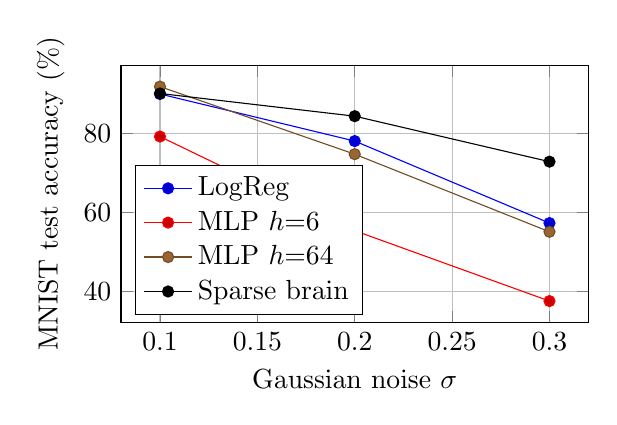
\begin{tikzpicture}
\begin{axis}[width=0.62\textwidth, height=0.4\textwidth, xlabel={Gaussian noise $\sigma$}, ylabel={MNIST test accuracy (\%)}, grid=both, legend pos=south west, legend cell align=left]
\addplot+[mark=*] coordinates {(0.10,90.05) (0.20,78.10) (0.30,57.28)};
\addplot+[mark=*] coordinates {(0.10,79.25) (0.20,55.35) (0.30,37.48)};
\addplot+[mark=*] coordinates {(0.10,91.93) (0.20,74.77) (0.30,55.07)};
\addplot+[mark=*] coordinates {(0.10,90.18) (0.20,84.42) (0.30,72.87)};
\legend{LogReg, MLP $h{=}6$, MLP $h{=}64$, Sparse brain}
\end{axis}
\end{tikzpicture}
\caption{Accuracy under additive Gaussian input noise (3 seeds). The saturating sparse core degrades more slowly than the ReLU baselines at high noise.}
\label{fig:noise}
\end{figure}
